\documentclass[hyperref={pdfpagelabels=false},mathserif,table,10pt]{beamer}
% File Name: SetUp.tex
% Function: Make main settings of the document.


%%%%%%%%%%%%%%%%%%%%%%%%%%% BEGIN-Theme-settings %%%%%%%%%%%%%%%%%%%%%%%%%%
%%%%% http://www.hartwork.org/beamer-theme-matrix/
\usetheme{default} % Set the theme of the beamer.
%\usetheme{Frankfurt}                     %% Geovani style
%\setbeamercolor{alerted text}{fg=blue}   %% Geovani style
% W/o������:default, boxes, Bergen, Madrid, Pittsburgh, Rochester
% ���������:Antibes, JuanLesPins, Montpellier��
% ��Ŀ¼(TOC)�IJ�ߵ�����: Berkeley, PaloAlto, Goettingen, Marburg, Hannover��
% ��΢��frame������:Berlin, Ilmenau, Dresden, Darmstadt, Frankfurt, Singapore, Szeged��
% ����С�ڱ���: Copenhagen, Luebeck, Malmoe, Warsaw��
%\usecolortheme{default}  % Outer color themes. Alternatives: whale, seahorse, dolphin. default, beaver
\usecolortheme{orchid}  % Inner color themes. Alternatives: lily, orchid.
\useinnertheme[shadow]{rounded}
\usefonttheme{structurebold} % Font themes. Alternatives:  default, serif, structurebold, structureitalicserif, structuresmallcapsserif
\setbeamertemplate{frametitle}
{   \begin{center}
        \insertframetitle
    \end{center}
}
\setbeamertemplate{itemize items}[default] % Alternatives: default/triangle, circle, square, ball
\setbeamertemplate{enumerate items}[default] % Alternatives: default, circle, square, ball
\setbeamertemplate{navigation symbols}{}
\setbeamertemplate{footline}[frame number]
%\setbeamertemplate{footline}{%
%  \leavevmode%
%  \hbox{%
%    \begin{beamercolorbox}[wd=.333333\paperwidth,ht=2.25ex,dp=1ex,center]{author in head/foot}%
%      \usebeamerfont{author in head/foot}\insertshortauthor~(\insertshortinstitute)
%    \end{beamercolorbox}%
%    \begin{beamercolorbox}[wd=.333333\paperwidth,ht=2.25ex,dp=1ex,center]{title in head/foot}%
%      \usebeamerfont{title in head/foot}\insertshorttitle
%    \end{beamercolorbox}%
%    \begin{beamercolorbox}[wd=.333333\paperwidth,ht=2.25ex,dp=1ex,right]{date in head/foot}%
%      \usebeamerfont{date in head/foot}\insertshortdate{}\hspace*{2em}
%      \insertframenumber{} / \inserttotalframenumber \hspace*{2ex}
%    \end{beamercolorbox}
%    }%
%  \vskip0pt%
%}
%%%%%%%%%%%%%%%%%%%%%%%%%%%% END-Theme-settings %%%%%%%%%%%%%%%%%%%%%%%%%%%


%%%%%%%%%%%%%%%%%%%%%%%%%%%%%% BEGIN-Packages %%%%%%%%%%%%%%%%%%%%%%%%%%%%%
\usepackage{amsmath,amssymb,amsfonts}
\usepackage{mathrsfs}
\usepackage{color,xcolor}
\usepackage{graphicx,subfigure}
\usepackage{clock} % Use this package to insert a clock in the beamer.
\usepackage{textcomp}
\usepackage[T1]{fontenc}
\usepackage{verbatim}
\usepackage{moreverb}
\usepackage{multirow,multicol}
%\usepackage{url}
%\usepackage[colorlinks,linkcolor=blue,citecolor=blue,urlcolor=blue]{hyperref}%[colorlinks,linkcolor=blue,citecolor=blue,urlcolor=blue]
\usepackage{CJK}
%%%%%%%%%%%%%%%%%%%%%%%%%%%%%%%% END-Packages %%%%%%%%%%%%%%%%%%%%%%%%%%%%%


% \setbeamertemplate{navigation symbols}{} % Disable the buttons at the bottom.

\graphicspath{{Figures/}} % Set the directory where figures are saved.

%\AtBeginSection{
%  \begin{frame}{Outline}
%    \tableofcontents[currentsection,hideallsubsections]
%  \end{frame}
%}
%\AtBeginSubsection{
%  \begin{frame}{Outline}
%    \tableofcontents[currentsection,currentsubsection]
%  \end{frame}
%}
\AtBeginSection{
  \begin{frame}{Outline}
  \large{
  \tableofcontents[sections={\thesection}]  }
  \end{frame}
}

%%%%%%%%%%%%%%%%%%%% BEGIN-Theorem-like Environments %%%%%%%%%%%%%%%%%%%%%
\newtheorem{mybox}{}
\newtheorem{Con}{Conjecture}[section]
\newtheorem{Thm}{Theorem}[section]
\newtheorem{Prop}{Proposition}[Thm]
% show fig and table number
\setbeamertemplate{caption}[numbered]
% show theorems and example number
\setbeamertemplate{theorems}[numbered]
%%%%%%%%%%%%%%%%%%%%% END-Theorem-like Environments %%%%%%%%%%%%%%%%%%%%%%


%%%%%%%%%%%%%%%%%%%%%%%%%% BEGIN-New Commands %%%%%%%%%%%%%%%%%%%%%%%%%%%%
\newcommand{\email}[1]{Email: \href{mailto: #1}{\tt {\color{blue}#1}}}
\newcommand{\red}{\color{red}}
\newcommand{\blue}{\color{blue}}
\newcommand{\brown}{\color{brown}}
\newcommand{\orange}{\color{orange}}
\newcommand{\yellow}{\color{yellow}}
\newcommand{\Real}{\mathbb{R}}
\newcommand{\Tran}[1]{#1^\mathrm{T}}
\newcommand{\st}{\textnormal{s.t.}}
\newcommand{\dist}{\textnormal{dist}}
\newcommand{\bc}{\begin{center}}
\newcommand{\ec}{\end{center}}
\newcommand{\tbf}{\textbf}
\newcommand{\be}{\begin{equation}}
\newcommand{\ee}{\end{equation}}
\newcommand{\ba}{\begin{array}}
\newcommand{\ea}{\end{array}}
\newcommand{\btab}{\begin{table}\begin{tabular}}
\newcommand{\etab}{\end{tabular}\end{table}}
\newcommand{\nn}{\nonumber}
\newcommand{\xn}{x_1,x_2,\ldots,x_n}
\newcommand{\framee}[2]{\frame{\frametitle{#1} #2}}
\newcommand{\reff}[1]{(\ref{#1})} % ������
\newcommand{\inner}[2]{\left\langle#1,#2\right\rangle}

%\renewcommand{\baselinestretch}{1.3}
% Ĭ��������룬������ó����˶���
\renewcommand{\raggedright}{\leftskip=0pt \rightskip=0pt plus 0cm}
\raggedright
%\large
% define Roman numbers
\makeatletter
\newcommand{\rmnum}[1]{\romannumeral #1}
\newcommand{\Rmnum}[1]{\expandafter\@slowromancap\romannumeral #1@}
\makeatother
%%%%%%%%%%%%%%%%%%%%%%%%%%%% END-New Commands %%%%%%%%%%%%%%%%%%%%%%%%%%%%


\begin{document}

\title[distance geometry]{\textsc{A New Error Function and Its Application in Distance Geometry Problem}}
\author[Zhenli SHENG]{Zhenli Sheng (ʢ����)\\email: {\blue szl@lsec.cc.ac.cn}}
% \institute{Institute of Computational Mathematics and Scientific/Engineering Computing}
\institute[ICMSEC, CAS]{Institute of Computational Mathematics and Scientific/Engineering Computing,\\Chinese Academy of Sciences}
\date[]{joint work with {\blue Prof. Ya-xiang Yuan} \\\textrm{} \\January 8, 2013\\ seminar talk}
\frame{
\titlepage
}

% File Name: ThankYou.tex
% Function: Insert an Outline page.


%\section*{\textsc{Outline}}
%\begin{frame}
%\frametitle{\textsc{Outline}}
%\end{frame}

\begin{frame}
\frametitle{\textsc{Outline}}
\tableofcontents%[pausesections]
\end{frame}


\section{Problem Introduction}
\frame{
\frametitle{Distance Geometry(DG) Problem}
Find the coordinate vectors $x_{1},x_{2},\ldots,x_{n}$ that satisfy several given distances between them. \\
\textrm{}\\
\begin{enumerate}[$\blacktriangleright$]
  \item<2-> data given:
        \begin{enumerate}[--]
          \item exact distances (error-free)
          \item inexact distances (with noises)
          \item distance bounds
        \end{enumerate}
        \textrm{}\\
        \textrm{}\\
  \item<3-> applications:
        \begin{enumerate}[--]
          \item graph realization
          \item {\red protein structure determination} (3D)
          \item sensor network localization (2D)
          \item ...
        \end{enumerate}
\end{enumerate}
}

\section{Related Works}
\frame{
\frametitle{Related works}
\begin{enumerate}[$\blacktriangleright$]
  \item<2-> Matrix Decomposition Method (Blumenthal 1953, Torgerson 1958)
  \item<3-> The Embedding Algorithm (Crippen, Havel 1988)
  \item<4-> Global Smoothing Algorithm (Mor\'{e}, Wu 1997)
  \item<5-> {\red Geometric Buildup Method} (Dong, Wu 2002)
  \item<6-> SDP Relaxiation Method (Ye, et al., 2006)
  \item<7-> ...
\end{enumerate}
}

\frame{
\frametitle{Matrix Decomposition Method}
{\red DG problem with full set of exact distances} \\
%\textrm{}\\
\small{
Given a full set of distances, $d_{i,j} = \| x_{i}-x_{j} \|, \quad i,j=1,2,\ldots,n.$ \\
\begin{enumerate}[$\blacktriangleright$]
  \item<2-> Set $x_{n} = (0,0,0\Tran)$, we have
      \begin{eqnarray}
      % \nonumber to remove numbering (before each equation)
        \nonumber d_{i,j}^{2} &=& \|x_{i}-x_{j}\|^{2} \\
        \nonumber             &=& \|x_{i}\|^{2}-2\Tran x_{i} x_{j}+\|x_{j}\|^{2} \\
                              &=& d_{i,n}^{2}-2\Tran x_{i} x_{j}+d_{j,n}^{2} \qquad  i,j=1,2,\ldots,n-1 \label{eq1}
      \end{eqnarray} \\
      \textrm{}\\
  \item<3-> Define $ X=(x_{1},x_{2},\ldots,x_{n}\Tran)$ and $D=\{(d_{i,n}^{2}-d_{i,j}^{2}+d_{j,n}^{2})/2: i,j=1,2,\ldots,n-1\}$,  (\ref{eq1}) $\Rightarrow {\red X\Tran X=D}$.\\
      \textrm{}\\
  \item<4-> Let $D=U\Sigma\Tran U$, and $V=U(:,1:3), \Lambda=\Sigma(1:3,1:3)$. Then $X = V\Lambda^{1/2}$ solves the problem. [{\blue Eckart and Young 1936}]
\end{enumerate} }
}

\frame{
\frametitle{Geometric Buildup Method}
\begin{enumerate}[$\blacktriangleright$]
  \item<2-> Find four atoms to form a base \\
        \begin{enumerate}[--]
          \item determine their coordinates to remove the possible translation and rotation/reflection
        \end{enumerate}
        \textrm{}\\
        \textrm{}\\
  \item<3-> Determine atoms one by one
        \begin{enumerate}[--]
          \item at least four distances from the undetermined atom to determined atoms are known
        \end{enumerate}
        \textrm{}\\
        \textrm{}\\
\end{enumerate}
\pause
\pause
\pause
\footnotesize{ Zachary Voller, Zhijun Wu(2012), {\blue Distance Geometry Methods for Protein Structure Determination.}}
}

\frame{
\frametitle{Determine one unknown atom}
Given four determined atoms $x_{1},x_{2},x_{3}$ and $x_{4}$, which $x_{i}=( x_{i1},x_{i2},x_{i3} \Tran)$ are known, and four {\orange exact} distances. \\
\begin{enumerate}[$\blacktriangleright$]
  \item<2-> $d_{i,j}^{2}=\|x_{i}\|^{2}-2\Tran x_{i} x_{j}+\|x_{j}\|^{2}  \qquad i=1,2,3,4.$
  \item<3-> $\Rightarrow {\red Ax_{j}=b},$ \\
        where
         $ A=2 \left(\begin{array}{ccc}
                    x_{11}-x_{21} & x_{12}-x_{22} & x_{13}-x_{23} \\
                    x_{21}-x_{31} & x_{22}-x_{32} & x_{23}-x_{33} \\
                    x_{31}-x_{41} & x_{32}-x_{42} & x_{33}-x_{43} \\
                    \end{array} \right)$ \\
         and
         $ b= \left( \begin{array}{c}
                       (\|x_{1}\|^{2}- \|x_{2}\|^{2}) -( d_{1,j}^{2}-d_{2,j}^{2} )\\
                       (\|x_{2}\|^{2}- \|x_{3}\|^{2}) -( d_{2,j}^{2}-d_{3,j}^{2} )\\
                       (\|x_{3}\|^{2}- \|x_{4}\|^{2}) -( d_{3,j}^{2}-d_{4,j}^{2} )
                     \end{array}
         \right). $ \\
  \textrm{}\\
  \textrm{}\\
  \item<4-> {\orange Inexact} distances?
\end{enumerate}
}

\frame{
\frametitle{Linear and Nonlinear Least-squares Approximation}
\small{
{\red DG problem with inexact distances}\\
%\textrm{} \\
Suppose $l$ distances between the unknown atom to the determined atoms are known.
\begin{enumerate}[$\blacktriangleright$]
  \item<2-> linear least-squares
            \begin{enumerate}[--]
              \item use only the $l$ distances
              \item $ \min \|b-Ax_{j}\|     $
            \end{enumerate}
%            \textrm{}\\
%            \textrm{}\\
  \item<3-> nonlinear least-squares
            \begin{enumerate}[--]
              \item use all the distances among the $l+1$ atoms
              \item solve a matrix decomposition problem
              \item move the same points in two different reference system coincide
            \end{enumerate}
            \footnotesize{  Atilla Sit, Zhijun Wu and Ya-xiang Yuan(2009), {\blue A geometric buildup algorithm for the solution of the distance geometry problem using least-squares approximation.}}
\end{enumerate} }
} 

\frame{
\frametitle{Laplacian Matrix}
\small{
Given a graph $(V,E)$, define its Laplacian matrix by L, whose entries $l_{i,j}$ are given by
\begin{enumerate}[$\blacktriangleright$]
  \item<2-> \begin{equation*}
             l_{i,j}=\left \{ \begin{array}{cll}
                      deg(v_{i}) & \textrm{if  } i=j, & \qquad  \rightarrow -sum(L(i,:))\\
                      -1         & \textrm{if  } (i,j)\in E, & \qquad \rightarrow {\red -exp(-d_{i,j}^{2}/2 ) }\\
                      0          & \textrm{otherwise}. &  \\
                              \end{array}
                     \right.
            \end{equation*}
            \textrm{}\\
            \textrm{}\\
  \item<3-> $L=D-A$, where D is degree matrix, and A is its adjacency matrix.
            \textrm{}\\
            \textrm{}\\
  \item<4-> Properties:
            \begin{enumerate}[--]
              \item L is always positive-semidefinite.
              \item 0 is always its eigenvalue and its corresponding eigenvector is $(1,1,\ldots,1\Tran)$.
              \item The number of times 0 appears as an eigenvalue in the Laplacian is the number of connected components in the graph.
            \end{enumerate}
\end{enumerate} }
}

\frame{
\frametitle{Eigenvector of smallest nonzero eigenvalue}
\begin{figure}[htp]
    \centering
    \subfigure{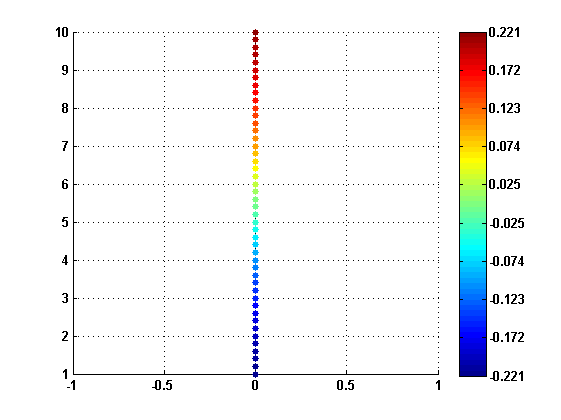
\includegraphics[width=4.5cm]{line.png} }
    \subfigure{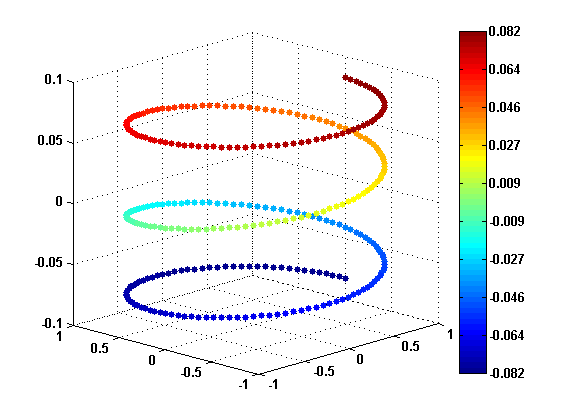
\includegraphics[width=4.5cm]{helix.png} }
    \subfigure{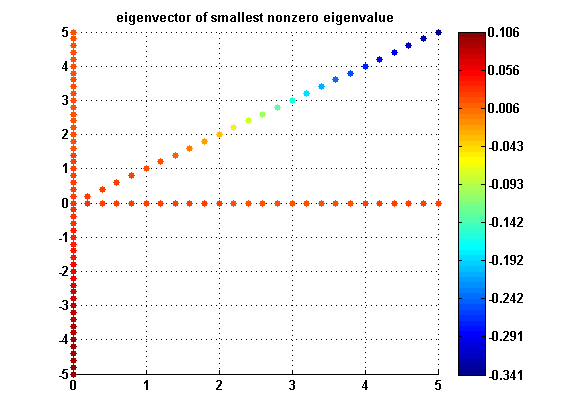
\includegraphics[width=4.5cm]{piecewise.png} }
    \subfigure{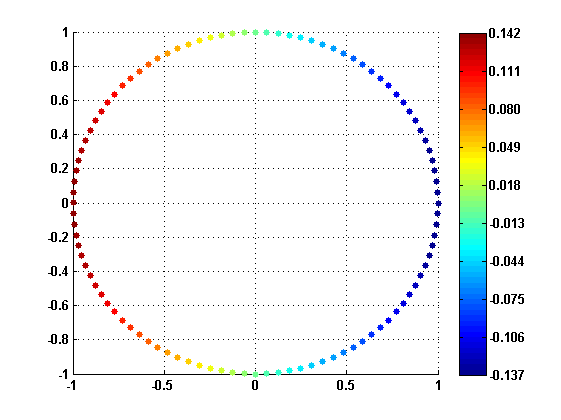
\includegraphics[width=4.5cm]{circle.png} }
\end{figure}
}

\frame{
\frametitle{a Conjecture}
\begin{Con}
Given a graph $(V,E)$, its Laplacian matrix is defined as before, then the eigenvector of the smallest nonzero eigenvalue, which can be viewed as a function of the vertexes, monotonically decrease or increase along the main trend/direction of the graph.
\end{Con}
\begin{figure}[htp]
  \centering
  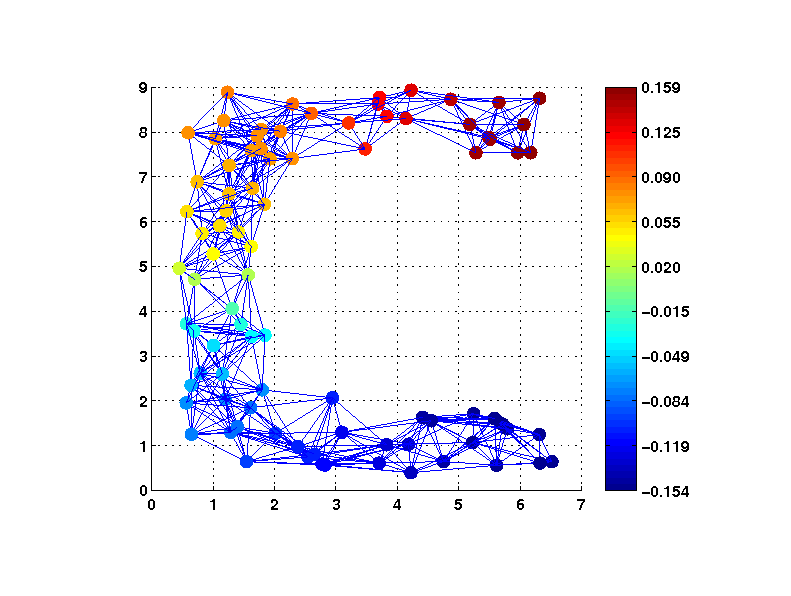
\includegraphics[width=6cm]{eigenone.png}
\end{figure}
}

\frame{
\begin{figure}[htp]
  \centering
  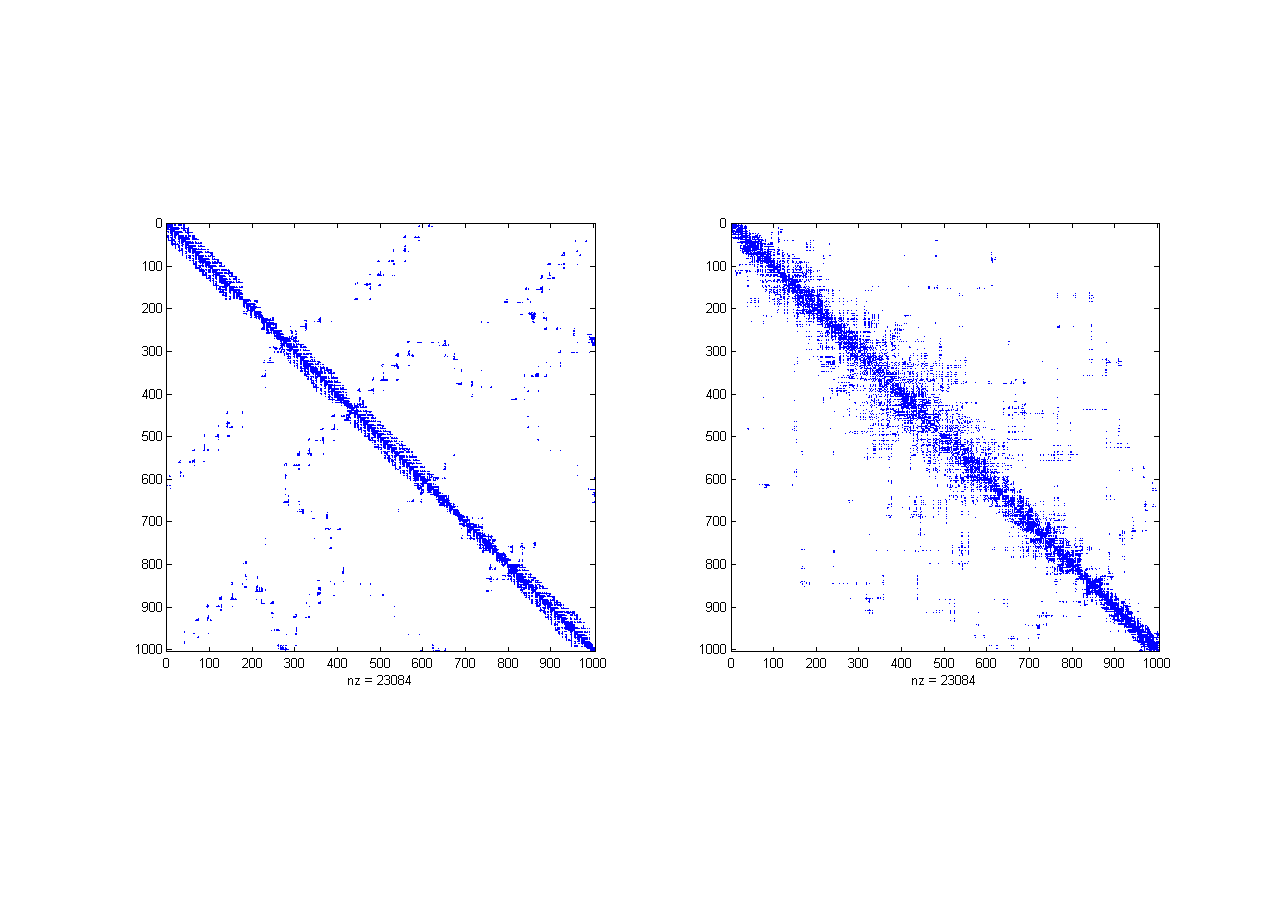
\includegraphics[width=10cm]{1AX8laplacian.png}
  \caption{1AX8}
\end{figure}
}

\frame{
\frametitle{Implement Details }
\begin{enumerate}[$\blacktriangleright$]
  \item<2-> computational order: \\
            \textrm{}\\
            \begin{center}
            \footnotesize{
            \begin{tabular}{|c|c|c|}
            % after \\: \hline or \cline{col1-col2} \cline{col3-col4} ...
              \hline
              \multicolumn{3}{|c|}{IAX8, 1003 atoms, cutoff=5{\AA}, 2.3\% exact} \\
              \hline
              order & RmsdErr & CPU time (s) \\
              \hline
              original & 7.395926e+000 & 1.258295 \\
              \hline
              greedy & 9.281000e-005 & 2.346640 \\
              \hline
              Laplacian & 9.281000e-005 & 1.999627\\
              \hline
              random & 7.372537e-007 & 4.980335 \\
                     & 1.726266e-007 & 2.946320 \\
                     & 3.858138e-003 & 2.988656 \\
                     & 2.437341e-008 & 3.517570 \\
                     & 1.223379e-005 & 4.757714 \\
                     & 1.169260e-003 & 5.339559 \\
                     & 1.399711e-006 & 2.478225 \\
                     & 1.771925e-005 & 4.957635 \\
                     & 9.559394e-009 & 2.750663 \\
                     & 8.637780e-007 & 5.196890 \\
              \hline
            \end{tabular} }
            \end{center}
  \end{enumerate}
}

\frame{
\begin{enumerate}[$\blacktriangleright$]
  \item computational order:\\
            \textrm{}\\
            \begin{center}
            \footnotesize{
            \begin{tabular}{|c|c|c|}
                \hline
                \multicolumn{3}{|c|}{1MQQ, 5681 atoms, cutoff=6{\AA}, 0.75\%, exact} \\
                \hline
                order & RmsdErr & CPU time (s) \\
                \hline
                original & 1.130061e+001 & 11.262673 \\
                \hline
                greedy & 4.310119e-003 & 53.904010 \\
                \hline
                Laplacian & 5.039401e-005 & 135.032459 \\
                \hline
                random & 5.315594e-003 & 23.218307 \\
                       & 1.612265e-002 & 67.657580 \\
                       & 2.928411e-004 & 142.834237 \\
                       & 2.262457e-007 & 29.632780 \\
                       & 3.823293e-006 & 70.646800 \\
                       & 3.165929e-003 & 140.470924 \\
                       & 8.535506e-001 & 254.812797 \\
                       & 6.665072e-005 & 214.758550 \\
                       & 4.334586e-001 & 141.894475 \\
                       & 2.888975e-001 & 23.932108 \\
                \hline
              \end{tabular} }
              \end{center}
\end{enumerate}
}

%\frame{
%\begin{enumerate}[$\blacktriangleright$]
%  \item computational order:\\
%  \footnotesize{
%    \begin{tabular}{|c|c|cc|cc|}
%      \hline
%      % after \\: \hline or \cline{col1-col2} \cline{col3-col4} ...
%      PDB ID & No. of atoms & RmsdErr & CPU time & RmsdErr & CPU time\\
%     \hline
%      1PTQ & 402 & 6.166615e+000 & 0.527040 & 4.801191e-011 & 3.236164 \\
%      1HOE & 558 & 3.469324e-004 & 0.468773 & 3.265660e-007 & 0.915511 \\
%      1LFB & 641 & 2.143626e-002 & 0.536184 & 2.517902e-006 & 0.910246 \\
%      1PHT & 811 &  &                       & 8.865440e-007 & 1.163034 \\
%      1POA & 914 & 1.009639e+001 & 1.071874 & 3.524817e-004 & 1.875779 \\
%      1AX8 & 1003 & 7.395926e+000 & 1.014269 & 9.281000e-005 & 2.039256 \\
%      1F39 & 1534 & 2.039362e+001 & 1.541356 & 6.742977e-005 & 3.904877\\
%      1RGS & 2015 & (5)4.570301e+003 & 1.874291 &(5)8.395178e+001 & 8.853443 \\
%      1KDH & 2923 & 2.096024e+001 & 2.787796 &(1)7.433055e+005 & 31.949689\\
%      1BPM & 3672 & (3)7.641587e+005 & 3.881272 &(6)3.217206e+005 & 24.251074\\
%      1RHJ & 3740 & 2.026798e+001 & 4.451570 & & \\
%      1HQQ & 3944 & (6)1.635136e+002 & 5.424702 & &\\
%      1TOA & 4292 & (12)2.647972e+001 & 5.086191 & &\\
%      1MQQ & 5681 & 2.313884e+004 & 7.136006 & &\\
%      \hline
%    \end{tabular} }
%\end{enumerate}
%}

\frame{
\begin{center}
\footnotesize{
\begin{tabular}{|c|c|ccc|c|ccc|}
  \hline
  % after \\: \hline or \cline{col1-col2} \cline{col3-col4} ...
  PDB ID & No. &  \multicolumn{3}{c|}{greedy order} &  & \multicolumn{3}{c|}{Laplacian order} \\
  \hline
         &     & RmsdErr & CPU time & NumDet & & RmsdErr & CPU time & NumDet \\
  \hline
    1PTQ & 402 & 1.15e-012 & 1.22e+000 & 402 & & 8.97e-013 & 4.98e-001 & 402 \\
    1HOE & 558 & 1.50e-012 & 8.09e-001 & 558 & & 1.08e-011 & 2.17e+000 & 558 \\
    1LFB & 641 & 7.59e-010 & 9.10e-001 & 641 & & 1.75e-010 & 1.51e+000 & 641 \\
    1PHT & 811 & 1.61e-011 & 1.23e+000 & 811 & & 1.67e-013 & 8.41e+001 & 4   \\
    1POA & 914 & 6.17e-010 & 1.43e+000 & 914 & & 3.31e-011 & 1.59e+000 & 914 \\
    1AX8 & 1003 & 1.24e-011 & 1.68e+000 & 1003 & & 4.87e-007 & 3.62e+000 & 1003 \\
    1F39 & 1534 & 2.32e-006 & 3.86e+000 & 1534 & & 4.03e-014 & 2.93e+002 & 1534 \\
    1RGS & 461  & 2.61e-014 & 2.11e-001 & 4    & & 3.33e-014 & 2.14e+000 & 4    \\
    1KDH & 2846 & 7.15e-004 & 8.56e+000 & 2846 & & 1.58e-001 & 5.17e+000 & 2846 \\
    1BPM & 3671 & 4.45e-005 & 9.03e+000 & 3671 & & 9.45e-013 & 9.92e+002 & 4    \\
    1RHJ & 3740 & 3.47e-008 & 1.07e+001 & 3740 & & 1.00e-006 & 1.19e+001 & 3740 \\
    1HQQ & 3944 & 4.77e-006 & 1.22e+001 & 3944 & & 2.76e+000 & 7.43e+000 & 3944 \\
    1TOA & 4292 & 2.35e+001 & 2.79e+001 & 4292 & & 1.09e-001 & 8.93e+000 & 4292 \\
    1MQQ & 5681 & 4.31e-003 & 4.98e+001 & 5681 & & 1.55e-002 & 5.48e+001 & 5681 \\
  \hline
\end{tabular} }
\end{center}
}

\frame{
\begin{figure}
  \centering
  \subfigure{ 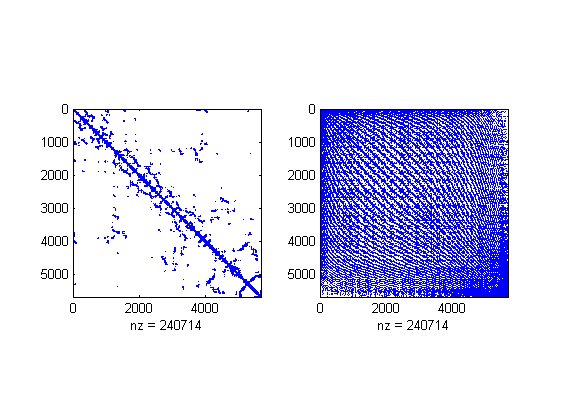
\includegraphics[width=5.5cm]{1MQQgreedyTheory.png} }
  \subfigure{ 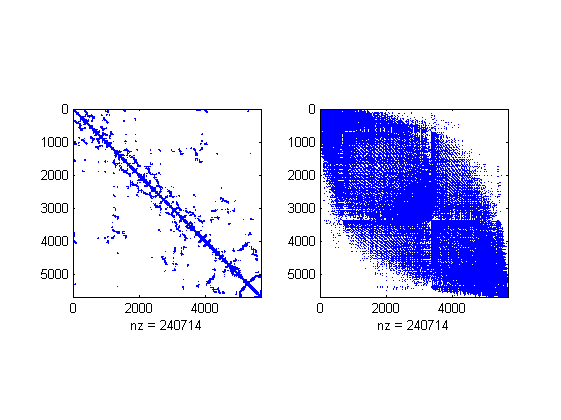
\includegraphics[width=5.5cm]{1MQQgreedyReal.png} }
  \caption{1MQQ, greedy, theoretical VS. real order}
\end{figure}
}

\frame{
\frametitle{Some other problems}
\begin{enumerate}[$\blacktriangleright$]
  \item<2-> not enough bases
  \item<3-> bad condition number: say, cond$(\Tran AA)>10^{6}$ \\
        $\Leftarrow$ bases almost in the same plane!
  \item<4-> $\rightsquigarrow$ move to last
\end{enumerate}
}

\section{Distributed Geometric Buildup Method}
\frame{
\frametitle{Motivation}

1MQQ, 5681 atoms, cutoff=6{\AA}, 0.75\%, exact distances \\
\begin{enumerate}[$\blacktriangleright$]
  \item<2-> {\red Error Accumulation!}
\end{enumerate}
\begin{center}  \footnotesize{
  \begin{tabular}{|c|c|c|c|}
     \hline
     Itr &   RmsdErr &     Itr &   RmsdErr \\
     \hline
     300 & 1.020647e-012 & 3000 & 1.186818e-004 \\
     600 & 1.805403e-010 & 3300 & 3.477342e-004 \\
     900 & 2.059775e-007 & 3600 & 1.953754e-003 \\
    1200 & 6.691896e-007 & 3900 & 1.973875e-003 \\
    1500 & 3.358551e-006 & 4200 & 2.162615e-003 \\
    1800 & 4.677271e-006 & 4500 & 2.231129e-003 \\
    2100 & 7.869284e-006 & 4800 & 2.790680e-003 \\
    2400 & 2.062700e-005 & 5100 & 3.084867e-003 \\
    2700 & 6.988388e-005 & 5400 & 4.277911e-003 \\
     \hline
   \end{tabular} }
\end{center}
}

\frame{
\frametitle{Divide and Conquer}
\begin{enumerate}[$\blacktriangleright$]
  \item<2-> Divide into small patches
  \item<3-> Geometric Buildup at each patch
  \item<4-> Stitch together
\end{enumerate}
}

\frame{
\frametitle{How to divide}
\begin{enumerate}[$\blacktriangleright$]
  \item<2-> {\blue symrcm}: minimize the bandwidth \\
        \footnotesize{  Pratik Biswas, Kim-Chuan Toh and Yinyu Ye(2007), {\blue A Distributed SDP Approach for Large-scale Noisy Anchor-free Graph Realization with Application to Molecular Conformation.}}
       \begin{figure}[htp]
             \centering
             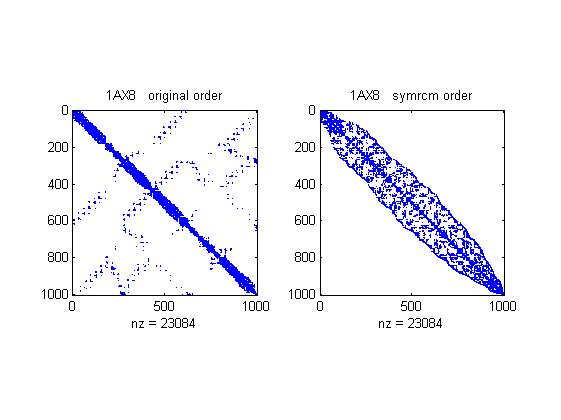
\includegraphics[width=10cm]{1AX8symrcm.png}
       \end{figure}
\end{enumerate}
}

\frame{
\frametitle{How to stitch}
Given two 3D point sets $\{p_{i}\}$ and $\{q_{i}\}$, $i=1,2,\ldots,k$.
\begin{enumerate}[$\blacktriangleright$]
  \item<2->  \begin{align}
               \nonumber \min_{R,T} \quad& \sum_{i=1}^{k} \| p_{i}- (Rq_{i}+T) \|_{2}^{2} \\
                         \st \quad & \Tran RR =I.
             \end{align}
  \item<3-> T: make their geometric center coincide
  \item<4-> R: \begin{align}\label{stitch}
                \nonumber \min_{R} \quad& \| P- RQ \|_{F}^{2} \\
                          \st \quad & \Tran RR =I.
               \end{align}
  Let $C=P\Tran Q$, and $C=U\Sigma\Tran V$, then $R=V\Tran U$ solves (\ref{stitch}).
  [{\blue Matrix Computation, Golub}]
  \item<5-> Remark: a fundamental problem in {\orange Machine Intelligence} and {\orange Optical Science}.
\end{enumerate}
}

\frame{
\frametitle{Numerical experiments}
Distributed Buildup:\\
\textrm{}\\
\textrm{}\\
\centering
\begin{tabular}{|c|c|cc|}
  \hline
  % after \\: \hline or \cline{col1-col2} \cline{col3-col4} ...
  PDB ID & No. of atoms & RmsdErr & CPU time \\
  \hline
  1PTQ & 402 & 1.781565e-012 & 0.912213  \\
  1HOE & 558 & 6.620519e-011 & 1.974754  \\
  1LFB & 641 & 4.849771e-012 & 1.660825  \\
  1PHT & 811 & 6.675090e-012 & 1.769367  \\
  1POA & 914 & 6.173696e-010 & 1.563789  \\
  1AX8 & 1003 & 4.161234e-008 & 1.793236 \\
  1F39 & 1534 & 3.480137e-012 & 4.303442 \\
  1RGS & 2015 & 1.804018e-009 & 4.713639 \\
  1KDH & 2923 & 5.424939e+002 & 18.708290 \\
  \hline
\end{tabular}
}

\section{Two New Models}
\frame{
\frametitle{A generalized DG problem}
{\red DG problem with distance bounds}  \\
\textrm{}\\
Given the lower bounds $l_{i,j}$ and upper bounds $u_{i,j}$, the problem can be formulated as:
\begin{align*}
  \max_{x_{i},r_{i}} \quad & \sum_{i=1}^{n} r_{i} \\
  \st                \quad & \|x_{i}-x_{j}\|+r_{i}+r_{j}\leq u_{i,j} \\
                           & \|x_{i}-x_{j}\|-r_{i}-r_{j}\geq l_{i,j} \qquad \forall (i,j)\in S\\
                           &  r_{i}\geq 0, \qquad i=1,2,\ldots,n.
\end{align*}
\footnotesize{Atilla Sit, Zhijun Wu(2011), {\blue Solving a Generalized Distances Geometry Problem for Protein Structure Determination. }}
}

\frame{
\frametitle{Matrix Completion for DG}
\begin{enumerate}[$\blacktriangleright$]
  \item<2-> Given distance matrix D, we have
             \begin{align*}
              DD=D.^{2} & =(d_{i,j}^2) \\
                        & =(\|x_{i}\|^{2}-2\Tran x_{i} x_{j}+\|x_{j}\|^{2}) \\
                        & =E+\Tran E-2X\Tran X.
             \end{align*}
            where E is a rank one matrix.
  \item<3-> rank(DD)=5.
  \item<4-> FPCA, LMaFit
\end{enumerate}
}

\frame{
\frametitle{A new type of MC problem}
\begin{enumerate}[$\blacktriangleright$]
  \item<2-> \begin{align*}
                \min_{X,x_{i}} \quad & \|X-\sum_{i=1}^{r}x_{i}\Tran x_{i} \|_{F}^{2} \\
                \st            \quad & X_{i,j} = M_{i,j}, \quad \forall(i,j)\in S, \\
                \end{align*}
  \item<3-> X is symmetric.
  \item<4-> M has some special structure (not randomly sampled).
\end{enumerate}
}


\section{Conclusions and Future work}
\frame{
\frametitle{Conclusions and Future work}
\begin{enumerate}[$\blacktriangleright$]
  \item<2-> What we have done:
        \begin{enumerate}[--]
          \item propose a distributed idea and a new possible way to divide
          \item propose a new model for DG
          \item finish some preliminary numerical experiments
        \end{enumerate}
        \textrm{}\\
        \textrm{}\\
  \item<3-> Future work:
        \begin{enumerate}[--]
          \item theoretical analysis on eigenvector of Laplacian matrix
          \item make clear the advantage and limitation of our distributed method
          \item work on the new models
        \end{enumerate}
\end{enumerate}
}

\frame{
\begin{center}
  \LARGE {\blue \textsc{Thank you for your attention!} }
\end{center}
}

\end{document}
